\chapter{Introduction}

%
% Vérifier intro problématique corpus
%
%
%%%%%%%%%%%%%%%%%%%%%%%%%%%%%%%%%%%%%%%%%%%%%%%%%%%%%%%%%%%%%%%%%%%%%%%%%%%%%%%%%%%%%%%%%%%%%%%%%%%%%%%%%%%%%%
% Présentation Contexte
% Présenter le projet, le contexte. GUIMUTEIC, caméra, visite, action utilisateur.
% Aide à l'utilisateur : réagir à l'intention de l'utilisateur, approt d'information sur ce qui est regardé
\section{Le Contexte de cette thèse}
%(Ajouter : on utilise indifféremment utilisateur ou visiteur).

Les sites touristiques, et notamment les musées, ont su assimiler les évolutions technologiques et proposer de nouvelles méthodes d'interaction pour enrichir les visites et les rendre davantage personnalisées.
La visite d'un site touristique peut être accompagnée d'un guide, qu'il s'agisse d'un humain (un guide culturel), ou d'une aide électronique.
Ces nouveaux outils, pouvant être mobiles ou fixes comme des bornes multimédia, ne remplacent pas un guide humain, mais permettent de fournir des informations visuelles (visio-guide) ou des informations audio (audio-guide), tout en réduisant la fatigue liée à la visite de musée sans aide~\cite{bitgood2009museum}.
Grâce aux avancées techniques, telles que la réduction de la taille des capteurs ou la puissance des processeurs mobiles, les possibilités des outils mobiles s'enrichissent. Et permettent même l'arrivée de solutions à base de réseaux de neurones profonds~\cite{howard2017mobilenets}.

Les guides électroniques permettent d'influencer les visites de musées, le visiteur restant plus longtemps et analysant plus en détail les œuvres~\cite{lanir2013influence}.
Malgré le fait qu'ils puissent, dans certains cas, gêner l'interaction sociale des visiteurs en groupes~\cite{lanir2013influence, grinter2002revisiting}, il est au contraire possible, grâce à un bon design, de promouvoir les échanges~\cite{gammon2008designing}.
En examinant les impacts des nouveaux usages des visiteurs~\cite{andreacola2014musee}, nous pouvons imaginer de nouvelles pratiques, avec notamment des visites plus personnalisées.
Que ce soit à travers la réalité augmentée ou l'identification automatique du contexte dans lequel se trouve l'utilisateur, ces systèmes reposent sur des procédés capables de reconnaître l'environnement qui entoure l'utilisateur.
Nous utiliserons dans la suite indifféremment utilisateur ou visiteur, car nous nous situons dans l'environnement de la visite de musées.

Cette thèse s'inscrit, avec un financement européen, dans le cadre d'un projet du Fonds Unique Interministériel (FUI) : Guide Multimédia de Tête, Informatif et Connecté (GUIMUTEIC).
Ce projet a pour but de proposer une nouvelle génération de guides pour les visites de musée.
Le dispositif GUIMUTEIC est équipé de différents capteurs, notamment une caméra.
Il est prévu pour être porté par chaque utilisateur et est destiné à enrichir la visite, en la personnalisant et en facilitant l'interaction.
Pour cela, le système GUIMUTEIC doit être capable d'identifier les points d'intérêts regardés par l'utilisateur, de le renseigner lorsque celui-ci le désire, et de réagir en fonction de ses actions.
Ce travail de thèse explore donc les besoins d'identification d'œuvres, d'actions et de l'environnement de l'utilisateur.



%\begin{figure}%
%\centering
%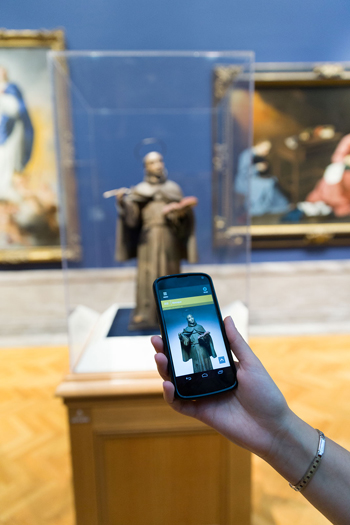
\includegraphics[width=\textwidth/3]{figures/ArtLens.jpg}%
%\caption{Exemple de visite avec une guide sur smartphone}%
%\label{fig:exemplevisite}%
%\end{figure}

\begin{figure}%
\centering
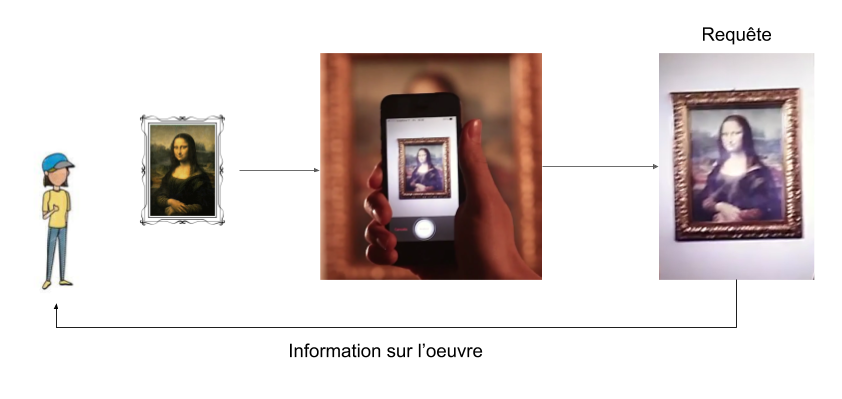
\includegraphics[width=\textwidth]{figures/Requete.png}%
\caption{Exemple d'une aide à la visite avec un smartphone. L'utilisateur peut prendre en photo une œuvre pour avoir des informations sur celle-ci.}
\label{fig:exemplevisitesmartphone}%
\end{figure}

%%%%%%%%%%%%%%%%%%%%%%%%%%%%%%%%%%%%%%%%%%%%%%%%%%%%%%%%%%%%%%%%%%%%%%%%%%%%%%%%%%%%%%%%%%%%%%%%%%%%%%%%%%%%%%
% PROBLEMATIQUE
% Reco d'oeuvre
% Reco d'action
% Reco de contexte
% Travail sur image et vidéo
\section{Problématiques de la recherche d'information muséale}
\label{sec:introcontraintes}
Les problématiques soulevées portent sur l'aide pouvant être apportée à l'utilisateur et les moyens d'interactions avec le dispositif mobile.
Équipé du dispositif GUIMUTEIC, intégrant une caméra embarquée, le but est de fournir à l'utilisateur une information sur son environnement, notamment les œuvres se trouvant face à lui.
Pour cela, il est nécessaire d'utiliser des méthodes d'identification d'instances précises.
Nous référons ici par ``{\it Instance}'', l'instance d'un objet, par exemple la Joconde, par opposition à une classe d'objet, dans ce cas un tableau.
Nous avons également besoin de déterminer si, et à quel moment, l'utilisateur désire avoir accès à de l'information à propos d’une œuvre.
En prenant comme exemple le musée de Bibracte\footnote{\url{http://www.bibracte.fr/}}, où certaines actions se déclenchent quand le visiteur entre dans une pièce, on comprend l'intérêt de réagir en fonction des actions de l'utilisateur.
La localisation de l’utilisateur seule n’est pas toujours suffisante lorsque l’on s’intéresse à identifier son environnement, en ne prenant pas en compte l’orientation ou ce à quoi l’utilisateur s’intéresse~\cite{schmidt1999there}.
C’est pourquoi nous allons nous intéresser à détecter des points d’intérêts que le visiteur regarde, en plus d’identifier ses actions grâce à de la détection de geste par le dispositif GUIMUTEIC.


%%%%%%%%%%%%%%%%%%%%%%%%%%%%%%%%%%%%%%%%%%%%%%%%%%%%%%%%%%%%%%%%%%%%%%%%%%%%%%%%%%%%%%%%%%%%%%%%%%%%%%%%%%%%%
% CONTRAINTES du projet
% Puissance limité
% Limitation sur les corpus
%\section{Contraintes du projet GUIMUTEIC}
%\label{sec:introcontraintes}
En dehors des problématiques scientifiques énoncées ci-dessus, ce travail s'inscrit dans le cadre d'un projet ``industriel''.
Ceci définit un certain nombre de contraintes qui vont influencer les choix effectués par la suite.
Tout d'abord, le système GUIMUTEIC est à destination de sites touristiques pouvant être de natures différentes, que ce soit en plein air ou en intérieur.
De même, le type des œuvres présentes dans un musée est très variable, de pierres taillées dans un musée d'archéologie, à des peintures ou des œuvres abstraites dans un musée d'art moderne, en passant par des voitures ou des pièces de monnaie.
L'objectif est de fournir une solution générale, pouvant s'adapter à chacun.

Une autre contrainte, directement liée au caractère industriel du projet, est l'effort de mise en place dans chacun des musées, qui doit être minimisé.
L'acquisition des données, la quantité de données recueillies ou l'annotation de ces données, sont des opérations coûteuses qui doivent être limitées.
L'objectif étant de proposer une solution applicable aisément à chaque musée, le travail demandé pour la mise en place doit être aussi réduit que possible.
L'étude de ces contraintes et de leurs impacts sur les choix pouvant être fait sera présentée dans le chapitre~\ref{chap:etude} intitulé~``\nameref{chap:etude}''.




%%%%%%%%%%%%%%%%%%%%%%%%%%%%%%%%%%%%%%%%%%%%%%%%%%%%%%%%%%%%%%%%%%%%%%%%%%%%%%%%%%%%%%%%%%%%%%%%%%%%%%%%%%%%%
% OBJECTIFS et CONTRIBUTION
\section{Contributions}

Les objectifs de cette thèse sont multiples : nous nous intéresserons à la reconnaissance d'instances et à l'exploration de différentes méthodes d'interaction avec l'utilisateur, tout en respectant les contraintes imposées par le projet GUIMUTEIC.


Ce travail de thèse apporte les contributions suivantes :
\begin{description}
	\item[Étude de l'accès à l'information pendant une visite touristique] La première contribution de ce travail de thèse concerne l'étude des visites de musées et les besoins en terme d'accès à l'information au cours des visites touristiques. Nous proposons un système mobile d'interaction entre l'utilisateur et le dispositif, qui permet de répondre aux attentes des musées et du projet GUIMUTEIC.
	\item[Reconnaissance d'instances] Nous proposons également une approche pour l'identification d'instances, dans le but de reconnaître les scènes vues par l'utilisateur. Pour cela, nous présentons un nouveau système de recherche d'image à base de réseaux de neurones siamois, pour l'apprentissage de similarité entre les images,.
	\item[Apprentissage des régions d'intérêt] Dans le but d'améliorer la reconnaissance d'instances, nous exposons une nouvelle méthode d'apprentissage automatique des régions d'intérêt dans les images. Cette méthode se base sur un apprentissage non supervisé des zones de l'image, et ne nécessite pas d'annotation de régions sur les images. Nous étudions l'apport de cette détection sur l'apprentissage de similarité, et comment apprendre les deux conjointement.
	\item[Détection de geste] Pour proposer une interaction avec l'utilisateur, nous cherchons à détecter ses gestes et actions grâce au dispositif GUIMUTEIC, c'est-à-dire avec une vue égocentrique (à la première personne). Nous développons pour cela un nouveau système de reconnaissance de gestes dans les vidéos à base de réseaux de neurones à convolutions, sans récursion.
	\item[Création de corpus d'évaluations] Pour vérifier la faisabilité du système développé dans des conditions réelles, nous avons recueilli plusieurs corpus dans les musées partenaires du projet. Tous les algorithmes développés dans cette thèse sont évalués sur ces corpus. La collecte et l'organisation de ces corpus sont présentées en annexe~\ref{chap:corpus} intitulée ``\nameref{chap:corpus}’’.
\end{description}


\subsection{Publications}

Le travail développé dans cette thèse à fait l'objet des publications suivantes :

\begin{itemize}
	\item \bibentry{portaz2018object}
	\item \bibentry{portaz2017fully}
	\item \bibentry{portaz2017construction}
	\item \bibentry{portaz2016etude}
	\item \bibentry{portaz2016mrim}
\end{itemize}

Le code développé ainsi que les collections créées dans cette thèse sont librement disponibles.
Pour le code utilisé pour les expérimentations, et également les schémas et les tableaux présentés, sont disponibles sur GitHub à l'adresse \url{https://github.com/maxgreat}.
Les collections d'images et de vidéos sont disponibles en accès libre dans le cadre de la recherche à l'adresse~\url{http://lig-mrim.imag.fr}.



%%%%%%%%%%%%%%%%%%%%%%%%%%%%%%%%%%%%%%%%%%%%%%%%%%%%%%%%%%%%%%%%%%%%%%%%%%%%%%%%%%%%%%%%%%%%%%%%%%%%%%%%%%%%%
% ORGANISATION de la thèse
\section{Plan du manuscrit}

Afin de décrire le travail mené dans le cadre de cette thèse nous suivons le plan suivant :


\begin{description}
	\item[Chapitre~\ref{chap:etude}:~\nameref{chap:etude}] Nous réalisons tout d'abord une étude approfondie du problème d'accès à l'information dans le cadre de visites touristiques.
Nous analysons plus en détail les contraintes spécifiques des musées.
Nous nous intéressons particulièrement aux différents moyens d'accès à l'information possibles dans ce contexte, et notamment aux types d'interactions avec l'utilisateur envisageables et désirables pour les visiteurs.

	\item[Chapitre~\ref{chap:stateoftheart}:~\nameref{chap:stateoftheart}] Nous introduisons différentes méthodes de recherche d'informations multimédia et d'analyse d'images existantes dans la littérature.
Nous présenterons l'état de l'art de la recherche d'images, particulièrement les techniques de réseaux de neurones profonds (Deep Learning).
Un état de l'art de la détection d'évènements dans les vidéos est aussi présenté.

	\item[\textbf{Chapitre~\ref{chap:similarite}:~\nameref{chap:similarite}}] Dans ce chapitre, nous présentons l'analyse et la modélisation du problème d'identification d'œuvres dans les images et vidéos.
Nous explorons différentes méthodes basées sur ce qui a été présenté dans le chapitre~\ref{chap:stateoftheart}, et nous les adaptons à nos problématiques. Nous évaluons ces méthodes sur les corpus d'images construits. 

\item[\textbf{Chapitre~\ref{chap:regions}:~\nameref{chap:regions}}] Nous fournissons une nouvelle méthode pour la détection de régions d'intérêt dans les images. Grâce à un apprentissage de la localisation des objets dans les images, sans annotation des régions sur le corpus d'apprentissage, nous obtenons des résultats supérieur à l'état de l'art sur nos collections. 

	\item[\textbf{Chapitre~\ref{chap:gestes}:~\nameref{chap:gestes}}] Ce chapitre est consacré à l'étude de la détection des actions de l'utilisateur dans les vidéos.
Suite à l'étude réalisée dans le chapitre~\ref{chap:etude}, nous nous intéressons aux gestes nécessaires à l'interaction et aux méthodes de détection possibles. Nous étudions la détection des gestes avec une vue à la première personne. Nous utilisons des réseaux de neurones non récursifs, avec pour objectif d'avoir un réseau de neurones compact et rapide, utilisable sur mobile. Nous évaluons notre approches grâce à un corpus de vidéos créé spécialement.

	\item[\textbf{Chapitre~\ref{chap:conclusion}:~\nameref{chap:conclusion}}] Finalement, le dernier chapitre présente la démarche générale. Nous concluons sur les contributions de ce travail de thèse, notamment sur les méthodes d'identifications d'instance et de détection de gestes à l'aide de réseaux de neurones profonds et sur la création du système GUIMUTEIC, ainsi que sur la suite des recherches possibles sur les problématiques présentées.

\end{description}




